\section{Diagramma Relazionale}
Procediamo ora con lo sviluppo del diagramma relazionale partendo dal concettuale, analiziamo nel dettagli tutte le scelte  implementative\footnote{ci concentreremo princpalmente sulle modifiche più radicali, molte entità infatti non verranno alterare} fatte in figura \ref{fig:diagrammaRelazionale}
\begin{figure}
    \centering
    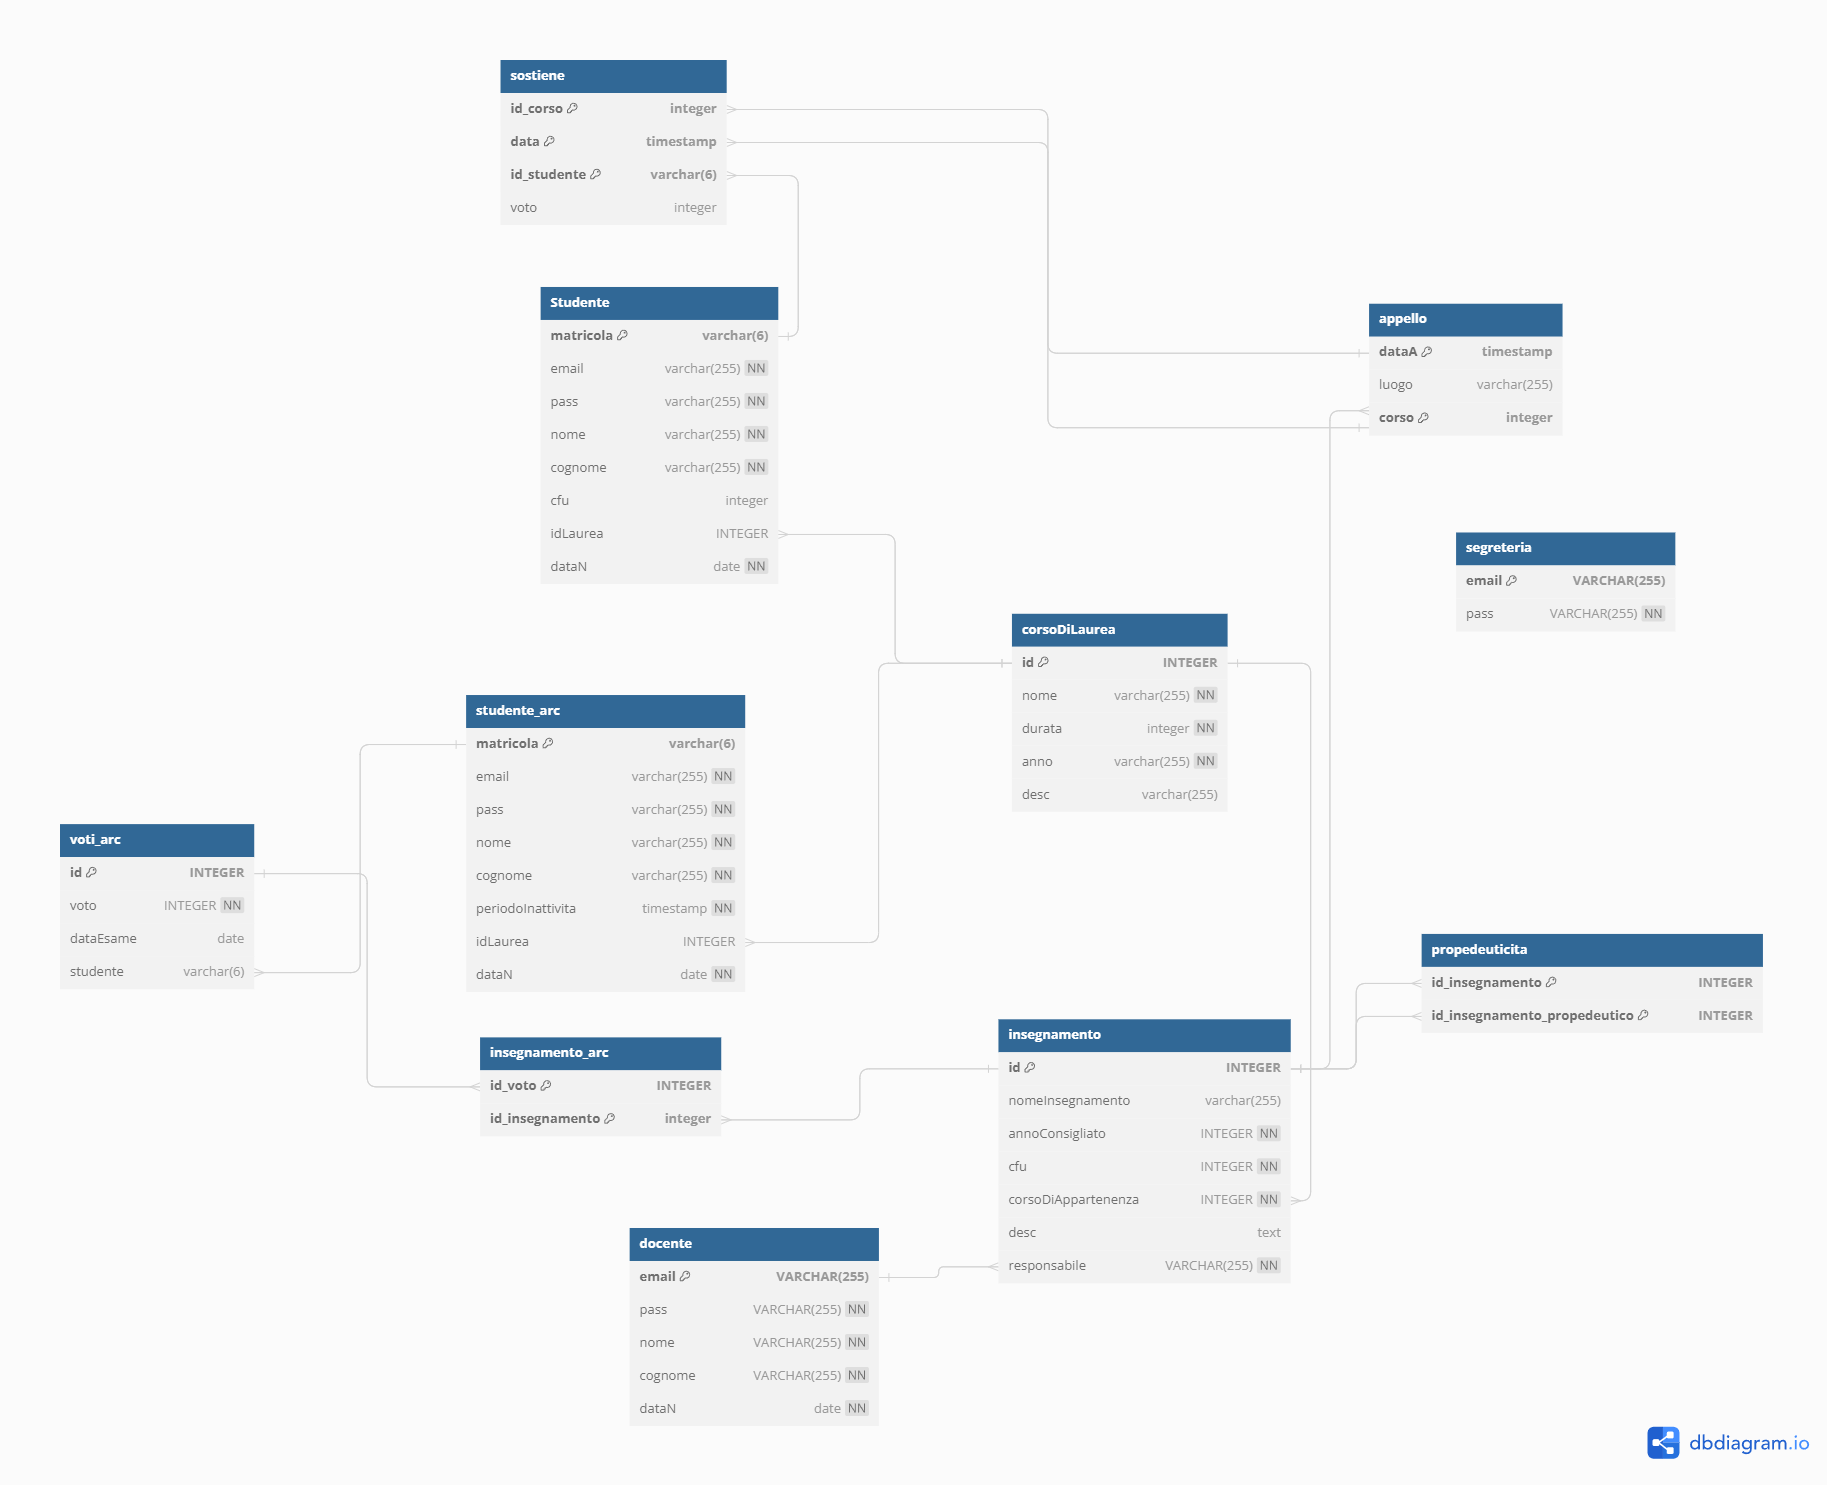
\includegraphics[width=0.9\linewidth]{images/relazionale.png}
    \caption{Diagramma Relazionale}
    \label{fig:diagrammaRelazionale}
\end{figure}
\subsection{Entità invariate}
Mostriamo ora le entità che non hanno ricevuto modifice significative: 
\begin{itemize}
    \item \textbf{corsoDiLaurea}: \underline{id} un integer auto increment che identifica il corso di laurea 
    \item \textbf{Studente}: la sua struttura rimane la stessa della sezione \ref{Studente} con la differenza che:
    \begin{itemize}
        \item \underline{matricola}: chiave primaria che identifica unviocamente lo studente  
        \item \dashuline{idLaurea}: chiave esterna riferita ad un corso di laurea che permette di identificare il corso di laurea a cui è iscritto 
    \end{itemize}
    \item \textbf{docente}: \underline{email} definisce unicovemente il docente con la struttura \textit{nome.cognomeN@segreteria.com}\footnote{dove \textit{N} definisce un numero intero generato tra 1,100}
    \item \textbf{Insegnamento}: 
    \begin{itemize}
        \item \textbf{id}  un integer auto increment che identifica l'insegnamento
        \item  \dashuline{responsabile}: chiave esterna che si riferisce all'insengnamente responsabile del corso, per motivi che illustreremo nello sezione \ref{createDocente} sarà fondamentale assegnare a responsabile un \textit{CONTRAINT DEFERRABLE INITIALLY DEFERRED}

    \end{itemize}
    \item \textbf{appello}:
    \begin{itemize}
        \item \underline{dataA}
        \footnote{dataA è chiave primaria in modo da rispettare il vincolo del singolo esame in un giorno per corso}
        : chiave primaria che rappresenta la data in cui viene sostenuto l'esame
        \item \dashuline{\underline{corso}} chiave primaria di appello e chiave esterna di insegnamento
    \end{itemize}
    \item \textbf{segreteria}: \underline{email} chiave primaria (vedi \ref{segreteria} per spiegazione)
\end{itemize}
\subsection{Moficiche}
Vediamo ora le entità che hanno subito cambiamenti radicali
\subsubsection{Gestione Archivio}
L'archivio è gestito da una serie da alcune entità che ora vedremo e analizzeremo nel dettaglio:
\begin{itemize}
    \item \textbf{studente\_arc}: \underline{email} stesso formato dello studente
    \item \textbf{voti\_arc}: \underline{id} definisce univicoamente il voto (vedi \ref{voto archivio})
    \item \textbf{insegnamento\_arc}:
    \begin{itemize}
        \item \dashuline{\underline{id\_voto}}: chiave primaria e chiave esterna su \textit{voti\_arc}
        \item \dashuline{\underline{id\_insengamento}}: chiave primaria e chiave esterna su \textit{insegnamento}
    \end{itemize}
    lo scopo di quest'entità emettere in relazione voti\_arc e insegnamento  in quanto essi hanno un rapporto n-n
\end{itemize}
\subsubsection{sostiene}
Quest'entità è forse quella che di più viene alterata, la sua struttua infatti diventa:
\begin{itemize}
    \item \dashuline{\textbf{id\_corso}}: chiave primaria e chiave esterna rispetto ad appello 
    \item \dashuline{\textbf{data}}:chiave primaria e chiave esterna rispetto ad appello 
    \item \dashuline{\textbf{id\_studente}}: chiave primaria e chiave esterna rispetto allo studente iscritto
\end{itemize}